\section{Supporting Materials}
% ==================================================================================================
\subsection{Notation}\label{app.notation}
Table~\ref{tab:notation} summarizes our notation,
and any corresponding parameters from \cite{Arenas2020}.
\begin{table}[ht]
  \centering
  \caption{Notation}
  \begin{tabular}{ccl}
  \toprule
   Symbol   &        Symbol        & Definition                     \\
   in this  & in \cite{Arenas2020} &                                \\
  \midrule
     $g$    &         $i$          & home patch                     \\
    $g'$    &         $j$          & other patch                    \\
    $g^*$   &         ---          & visited patch                  \\
     $a$    &         $g$          & self age group                 \\
    $a'$    &         $h$          & other age group                \\
     $y$    &         ---          & contact type                   \\
     $n$    &         ---          & home FSA                       \\
    $n'$    &         ---          & visited FSA                    \\
     $i$    &         $m$          & infection state                \\
     $P$    &         $N$          & population size                \\
     $B$    &         $R$          & mobility matrix                \\
     ---    &         $M$          & convenience mobility matrix    \\
  $\lambda$ &        $\Pi$         & force of infection             \\
   $\rho$   &         $p$          & mobility factor                \\
     $h$    &         ---          & home pool contact proportion   \\
     $C$    &         $k$          & contacts per person            \\
     $X$    &         ---          & total absolute contacts        \\
  $\theta$  &         $C$          & contacts age distribution      \\
   $\phi$   &         ---          & odds of mobility if unobserved \\
   $\psi$   &         ---          & relative time away from home   \\
  \bottomrule
\end{tabular}
  
  \label{tab:notation}
\end{table}
% ==================================================================================================
\subsection{Interpretation of ``Non-mobile''}\label{app.non-mob}
% SM: love this section and its examples which are clear and powerful
As described in \S~\ref{meth.orig}, \citet{Arenas2020} model the degree of mobility of age group $a$
using a parameter $\rho_a$ (our notation),
incorporated into a convenience matrix $M_{gg'}$ per Eq.~(\ref{eq:Arenas.M})\,/\,(\ref{eq:Arenas.M.app}),
repeated here for reference:
\begin{equation}\label{eq:Arenas.M.app}
  M_{gg'a} = (1-\rho_a)\,\delta_{gg'} + \rho_a B_{gg'a}
\end{equation}
The implicit assumption of this approach is that
non-mobile individuals may form contacts with visitors to the former's residence patch
(situation~\ref{situ:mob-at-home} in \S~\ref{meth.prop.mix.mob}):
an assumption which may not be desired depending on the research question or intervention effect.
The proposed approach to modelling mixing can avoid this assumption if needed
through the use of ``home pools'' (situation~\ref{situ:non-mob}).
Figure~\ref{fig:nm} explores the potential influence of this assumption on network connectivity,
% SM: clarify what "this" refers to (the original assumption?)
as measured by the expected proportion of contacts formed with other patches, in a toy example.
The example has 3 patches, each having equal population size and random mobility ($B_{gg'} = 1/N_{g'}$).
Age is not considered.
\par
By simulating mixing between non-mobile individuals and mobile visitors
(Figures~\ref{fig:nm.half.stay}~\&~\ref{fig:nm.diff.stay}, situation~\ref{situ:mob-at-home})
% SM: minor point - the greying out of "travel pool" label, etc.
% may need to be a few shades darker to read on some screens.
% these figures are +++stunning and clear!
% I also really like the use of the figures to demonstrate the examples
the proportions of contact made with other patches increases for all patches,
as compared to the proposed approach
(Figures~\ref{fig:nm.half.home}~\&~\ref{fig:nm.diff.home}, situation~\ref{situ:non-mob}).
The difference is largest in the context of differential mobility by patch
% SM: here, refer to issue 2? and also could refer back to its implications
% v. briefly (differential mobility by age, but also other contexts...)
(Figures~\ref{fig:nm.diff.stay}~vs~\ref{fig:nm.diff.home}).
\par
\begin{figure}[ht]
  \newcommand{\threepct}[3]{#1,~#2,~#3\,\%}
  \centering
  \begin{subfigure}{0.49\linewidth}
    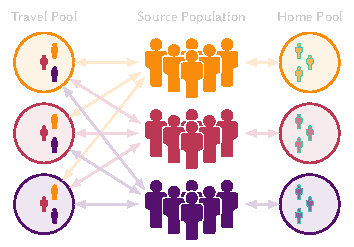
\includegraphics[width=\linewidth]{pools-half-home}
    \caption{Non-mobile = stay at home, all patches 50\% mobile}
    \label{fig:nm.half.home}
    \floatfoot{Contacts formed with other patches:\\
      33\% if non-mobile have equal contact rates vs mobile\\
      44\% if non-mobile have 1/2 contact rates vs mobile}
  \end{subfigure}\hfill%
  \begin{subfigure}{0.49\linewidth}
    \centering
    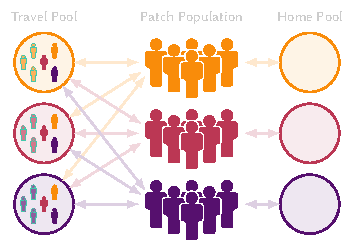
\includegraphics[width=\linewidth]{pools-half-stay}
    \caption{Non-mobile = stay in patch, all patches 50\% mobile}
    \label{fig:nm.half.stay}
    \floatfoot{Contacts formed with other patches:\\
      50\% if non-mobile have equal contact rates vs mobile\\
      59\% if non-mobile have 1/2 contact rates vs mobile}
  \end{subfigure}\medskip\par
  \begin{subfigure}{0.49\linewidth}
    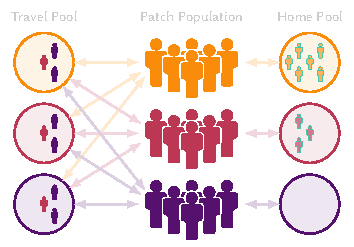
\includegraphics[width=\linewidth]{pools-diff-home}
    \caption{Non-mobile = stay at home, patches \threepct{0}{50}{100} mobile}
    \label{fig:nm.diff.home}
    \floatfoot{Contacts formed with other patches:\\
      \threepct{0}{33}{33} if non-mobile have equal contact rates vs mobile\\
      \threepct{0}{44}{33} if non-mobile have 1/2 contact rates vs mobile}
  \end{subfigure}\hfill%
  \begin{subfigure}{0.49\linewidth}
    \centering
    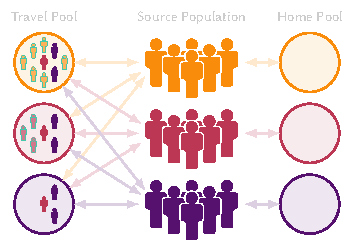
\includegraphics[width=\linewidth]{pools-diff-stay}
    \caption{Non-mobile = stay in patch, patches \threepct{0}{50}{100} mobile}
    \label{fig:nm.diff.stay}
    \floatfoot{Contacts formed with other patches:\\
      \threepct{33}{48}{59} if non-mobile have equal contact rates vs mobile\\
      \threepct{50}{58}{52} if non-mobile have 1/2 contact rates vs mobile}
  \end{subfigure}
  \caption{Mixing implications for two assumptions about the behaviour of non-mobile populations:
    ``stay at home'' (\subref{fig:nm.half.home},\subref{fig:nm.diff.home},
    reflecting situation~\ref{situ:non-mob}):
    % SM: in main text, sometimes referred to as issue 3, etc...
    % suggest either situation or issue for consistency...
    no contacts with other patches (proposed here); vs
    ``stay within patch'' (\subref{fig:nm.half.stay},\subref{fig:nm.diff.stay},
    reflecting situation~\ref{situ:mob-at-home}):
    no travel, but may form contacts with travellers from other patches (as in \cite{Arenas2020}).}
  \floatfoot{
    Non-mobile populations are indicated with faded colour and green outline;
    patch-specific values ordered from top (yellow) to bottom (purple).
    Additional assumptions:
    large population size;
    equal population sizes and contact rates by patch;
    random mobility (equal probability of visiting any patch if mobile).}
  \label{fig:nm}
\end{figure}
\clearpage
% ==================================================================================================
\subsection{Deriving the Mobility Matrix: Example}\label{app.mob}
% SM: this is great. I like that you outlined each step and put it here - it was a lot of work,
% and is nice to be transparent but also enable its use by others
% who can request/work with similar cell phone data, etc.
Here we describe the methods used to obtain the mobility matrix $B_{gg'}$
for our applied example in Ontario Canada (details in \S~\ref{ex}).
The mobility matrix represents
the expected proportions of individuals residing in decile (patch) $g$ who travel to decile $g'$ each day.
We will begin by producing the FSA-level mobility matrix $B_{nn'}$ ($513 \times 513$),
and later aggregate this matrix to obtain $B_{gg'}$ ($10 \times 10$).
% --------------------------------------------------------------------------------------------------
\subsubsection{Data}\label{app.mob.data}
The raw data represent logs of: timestamp, geolocation (latitude\,/\,longitude), and unique device ID.
% SM: cite a paper by Amir if possible where he used these types of data
A log entry (``ping'') is generated when an app on the device
requests the current geolocation from the service provider.
Geolocation is logged using Geohash level 6 (1.2 \,km $\times$ 609.4\,m).
The midpoint of each Geohash is then compared to boundary files representing all 513 Ontario FSAs%
\footnote{\hreftt{https://www150.statcan.gc.ca/n1/en/catalogue/92-179-X}}
to determine which FSA the ping is attributed to.
The following definitions were then used to determine device mobility.
\begin{itemize}
  \item \textbf{Home FSA:} for each unique device,
  the FSA with the greatest daily-average time between 8:00\,pm--5:00\,am during each calendar month.
  Devices for which it was not possible to determine the home FSA were excluded from all further analysis.
  \item \textbf{Visited FSA:} FSAs that a device travelled to within a 24-hour period,
  as defined by at least 2 consecutive pings spanning at least 2 hours within the FSA.
  By this definition, it was possible for a device to visit multiple FSAs, or no FSA during a given day.
  Repeated visits to the same FSA by the same device on the same calendar date are treated as a single visit.
  \item \textbf{Time away from home:} the proportion of time each device
  % SM: for some reason I thought it was % of devices that were away from home for X period of time
  % [like at least 1 hour, etc.]? but I think you have already double-checked this with Amir?
  was estimated to be away from the home dwelling (not just home FSA).
  The home dwelling was defined by the Geohash 6 tile
  with the greatest daily-average time between 8:00\,pm and 5:00\,am each month.
% MH: Given you have already defined home FSA above think this is unneccessary.
% JK: Hm, but the definition of dwelling has not been introduced?
% actually, I also need AG to confirm this detail.
% MH: Also reads as if the "time away from home" is defined by
% the greatest daily average time between 8:00pm  to 5:00am each month.
% JK: good point this though, I edited a bit to clarify.
\end{itemize}
\par
These definitions were applied to each calendar month $t$ from Jan 2020--Dec 2020 (12 months) to compute:
the mean number of devices with home FSA $n$ per day, denoted $H_{nt}$ or ``observed devices'';
the mean number of devices with home FSA $n$ that visited FSA $n'$ per day, denoted $V_{nn't}$, or ``device visits''; and
the mean proportion of time each device spent outside the home per day for each FSA, denoted $W_{nt}$.
% --------------------------------------------------------------------------------------------------
\subsubsection{Inter-FSA Mobility}\label{app.mob.inter}
The inter-FSA mobility matrix $B_{nn't}$ ($n \ne n'$) could be defined as
the proportion of observed devices that travelled to each FSA ($V_{nn't} / H_{nt}$).
However, the following analysis of the data suggested that such an approach may bias estimates of mobility.
A reference period $t_0$ was defined as Jan--Feb 2020, to reflect pre-pandemic conditions.
The expected values of $H_{nt}$ and $V_{nt} = \sum_{n' V_{nn't}}$ for each FSA during this period were then
computed and compared to the expected values during each subsequent month.
Figure~\ref{fig:RHVt} plots the distribution of ratios
$H_{nt} / H_{nt_0}$ (\subref{fig:RHt}) and $V_{nt} / V_{nt_0}$ (\subref{fig:RVt})
across all 513 FSAs, for each month.
These ratios illustrate that both $V_{nt}$ and $H_{nt}$ were influenced (reduced) by pandemic restrictions,
and thus $V_{nn't} / H_{nt}$ would overestimate mobility.
The trend in $H_{nt}$ might be because apps accessing geolocation services are only opened
after the user intends to travel, such as map-related apps.
\begin{figure}
  \centering
  \begin{subfigure}{0pt}\refstepcounter{subfigure}\label{fig:RHt}\end{subfigure}%
  \begin{subfigure}{0pt}\refstepcounter{subfigure}\label{fig:RVt}\end{subfigure}%
  \begin{subfigure}{0pt}\refstepcounter{subfigure}\label{fig:RH0Vt}\end{subfigure}%
  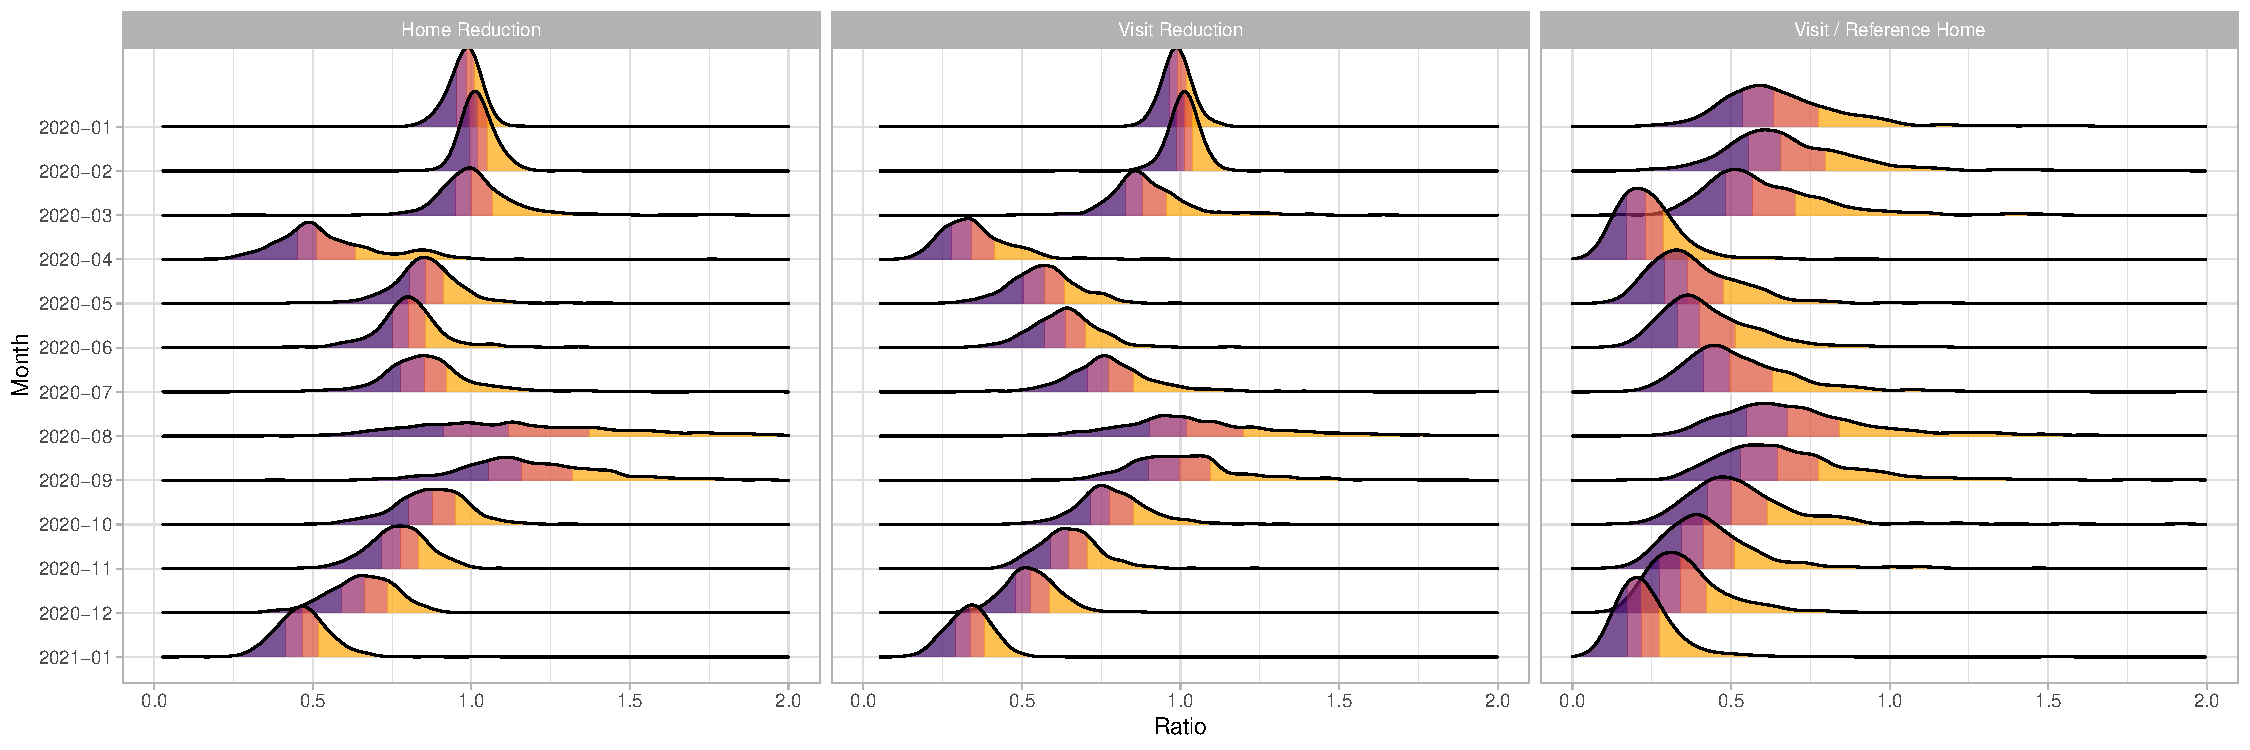
\includegraphics[width=\linewidth]{devices-ratios}
  \caption{Ratios of (\subref{fig:RHt}) observed devices at home
    and (\subref{fig:RVt}) total device visits
    during each month versus during the reference period
    suggesting that the proportion of observed devices travelling each month
    alone is not reflective of true mobility or else (\subref{fig:RHt}) would be 1;
    (\subref{fig:RH0Vt}) adjusted mobility measure: ratio of
    device visits each month from versus
    the number of observed devices at home during the reference period}
  \label{fig:RHVt}
  \floatfoot{Data from approximately 2\% of mobile devices in Ontario, Canada;
    distributions show the density of ratio values across all 513 FSAs;
    coloured segments indicate the 4 quantiles of each distributions;
    reference period: Jan--Feb 2020.}
\end{figure}
\par
To address the above measurement bias, we chose $H_{nt_0}$ as a more reliable denominator,
and thus modelled mobility using: $V_{nn't} / H_{nt_0}$ (Figure~\ref{fig:RH0Vt}).%
\footnote{One limitation of this approach is that the reference period only includes winter months,
  which may not be representative of mobility year-round or seasonal variablity in mobility.
  Indeed, all three ratios in Figure~\ref{fig:RHVt} have substantial tails above 1 during Aug--Sept 2020,
  suggesting that mobility was higher during that period versus the pre-pandemic reference period.}
The results of Figure~\ref{fig:RHVt} also suggest that
unobserved devices are less mobile than observed devices;
thus the unobserved devices would not have the same expected mobility as the observed devices.
To account for this observation, we first estimated the total number of devices per FSA, denoted $D_n$,
using Statistics Canada data on smart-phone ownership by age group.%
\footnote{\hreftt{https://www150.statcan.gc.ca/t1/tbl1/en/tv.action?pid=2210011501}}
Based on these data, we estimate that $H_{nt}$ represents
2.2~[IQR:~1.9,~2.6]\,\% of devices pre-pandemic, and
1.8~[IQR:~1.4,~2.3]\,\% after from March 2020--Jan 2021.
The number of unobserved devices in FSA $n$ before the pandemic is therefore $D_n - H_{nt_0}$.
\par
During the pandemic, additional devices go unobserved ($H_{nt}$ decreases)
but we assume that the newly unobserved devices do not travel.
Therefore, the number of devices that may travel unobserved
is a proportion of $D_n - H_{nt_0}$, not a proportion of $D_n - H_{nt}$.
Since we have no data on unobserved individuals, we assume that they are mobile
% SM: 'these' refers to unobserved individuatls?
at a rate $\phi_1 \le 1$ (default 0.9) relative to the observed devices.
Similarly, for individuals who do not own devices ($P_n - D_n$) we assume that they are mobile
at a rate $\phi_2 \le 1$ (default 0.9) relative to the observed devices.
We assume $\phi_1 \le 1$ and $\phi_2 \le 1$ because, as noted above,
the trends in Figure~\ref{fig:RHt} suggest that
individuals are more likely to be observed via geolocation pings after forming an intention to travel.
Thus, the total proportion of individuals in FSA $n$ who travel to FSA $n'$ during month $t$ is modelled~as:
\begin{equation}\label{eq:Bnnt.inter}
  B_{nn't \,(n\ne n')} = \frac{V_{nn't}}{H_{nt_0}} \big[
  \underbrace{1\vphantom{\phi}}_{\textrm{(a)}}
  + \underbrace{\phi_1 \left(D_n - H_{nt_0}\right)}_{\textrm{(b)}}
  + \underbrace{\phi_2 \left(P_n - D_n\right)}_{\textrm{(c)}} \big] P_n^{-1}
\end{equation}
where (a) represents the observed devices,
(b) unobserved devices, and
(c) individuals without devices.
% --------------------------------------------------------------------------------------------------
\subsubsection{Intra-FSA Mobility}\label{app.mob.intra}
Since device visits to other FSA $V_{nn't}$ do not include ``visits'' within the home FSA,
the proportion of individuals who are mobile (making contacts) within their home FSA is not yet determined.
During the reference period, we assume that
all individuals who do not travel to other FSAs are still mobile within their home FSA:
\begin{equation}\label{eq:Bnnt.intra.t0}
  B_{nn't_0\,(n = n')} = 1 - \sum_{n'} B_{nn't_0\,(n \ne n')}
\end{equation}
During pandemic months, we assume that
a proportion of such individuals remain mobile within their home FSA;
this proportion is derived using the time away from home $W_{nt}$ as follows.
% SM: refer back to Section A.3.1. here
We assume that individuals who are mobile within their home FSA
spend $\psi \le 1$ (default 1) as much time away from home as
those who travel to other FSAs.
Thus, the model for $W_{nt}$ is:
\begin{equation}\label{eq:Wnt}
  W_{nt} = W^*_n \left(\psi B_{nn't\,(n = n')} + \sum_{n'} B_{nn't\,(n \ne n')} \right)
\end{equation}
where $W^*_n$ is the expected proportion of time away from home
among travellers from FSA $n$ to other FSAs.
During the reference period, all individuals are mobile so $B_{nn't_0\,(n = n')} = 0$ is known, and
$W^*_n$ can be calculated by rearranging Eq.~(\ref{eq:Wnt}).
Then, during the pandemic months, the observed $W_{nt}$ can be used to infer $B_{nn't\,(n = n')}$
by rearranging again:
\begin{equation}\label{eq:Bnnt.intra.t}
  B_{nn't\,(n = n')} = \left(\frac{W_{nt}}{W^*_n} - \sum_{n'} B_{nn't\,(n \ne n')}\right) \psi^{-1}
\end{equation}
Figure~\ref{fig:W} plots the distribution of expected times away from home $W_{nt}$
in hours (\subref{fig:W-hours}) and relative to the reference period $W_{nt_0}$ (\subref{fig:W-relative}).
\par
During the pandemic months, $B_{nn't}$ will sum to less than 1 for many FSAs;
this is desirable, since we interpret $1 - \sum_{n'} B_{nn't}$ as
the expected proportion of individuals in FSA $n$
who did not leave the home each day during month~$t$,
and thus would not form any mobility-related contacts.
Similarly, if $B_{nn't}$ sums to greater than 1, the net result in the force of infection is that
individuals may form more contacts than expected from the reference period,
which is also usually acceptable (such as during Aug--Sept 2020).
\begin{figure}
  \centering
  \begin{subfigure}{0.4\linewidth}
    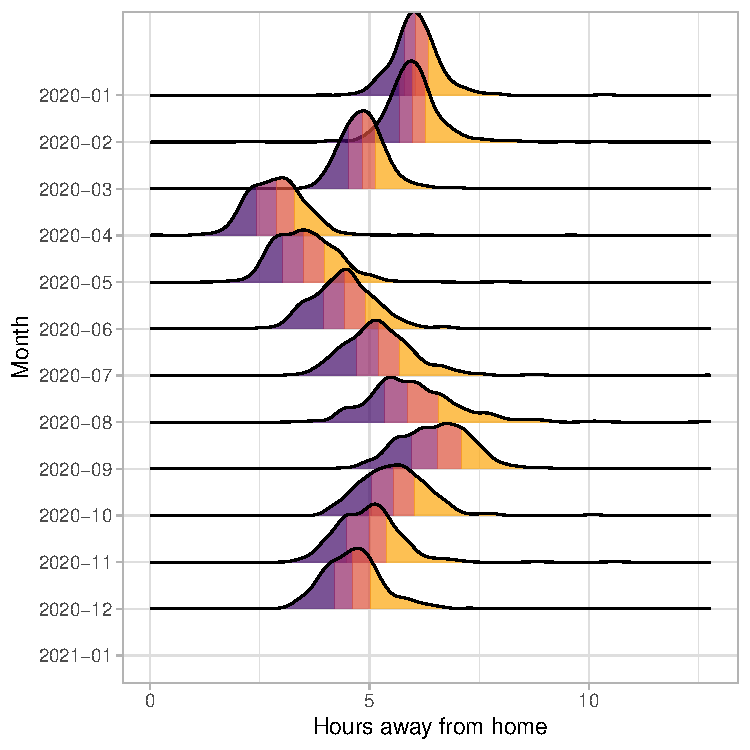
\includegraphics[width=\linewidth]{t-away-hours}
    \caption{Hours away from home}
    \label{fig:W-hours}
  \end{subfigure}
  \begin{subfigure}{0.4\linewidth}
    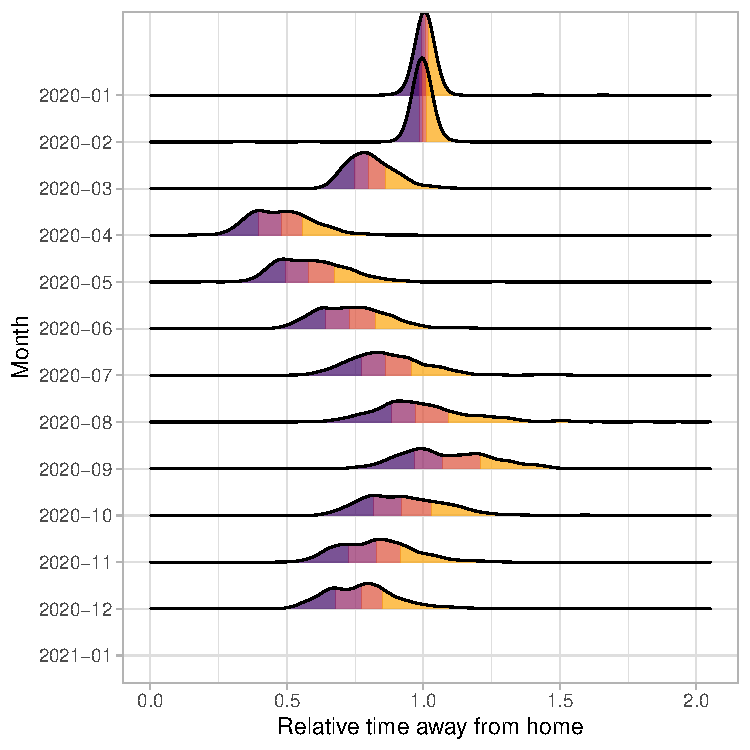
\includegraphics[width=\linewidth]{t-away-relative}
    \caption{Relative time away versus reference period}
    \label{fig:W-relative}
  \end{subfigure}
  \caption{Expected time away from home in hours and relative to the reference period}
  \label{fig:W}
  \floatfoot{Data from approximately 2\% of mobile devices in Ontario, Canada;
    distributions show the density of ratio values across all 513 FSAs;
    coloured segments indicate the 4 quantiles of each distributions;
    reference period: Jan--Feb 2020.}
\end{figure}
\par
Finally, as noted in \S~\ref{ex:data}, Eq.~(\ref{eq:Bgg})\,/\,(\ref{eq:Bgg.app})
can be used to aggregate $B_{nn'}$ to obtain $B_{gg'}$ (repeated here for reference):
\begin{equation}\label{eq:Bgg.app}
  B_{gg'} = \sum_{n \in S_g}\sum_{n' \in S_g'} B^h_{nn'}
\end{equation}
where $S_g$ is the set of FSAs ($n$) corresponding to decile $g$.
Figure~\ref{fig:Bggt} illustrates the monthly matrices $B_{gg't}$ for the study period
with and without the inferred mobility within the home decile.
Mobility patterns outlined in Figure~\ref{fig:Bggt} are generally consistent across months,
with the overall proportions of travelling individuals
proportional to the ratio $V_{nn't} / H_{nt_0}$ depicted in Figure~\ref{fig:RH0Vt}.
\begin{figure}[ht]
  \centering
  \begin{subfigure}{\linewidth}
    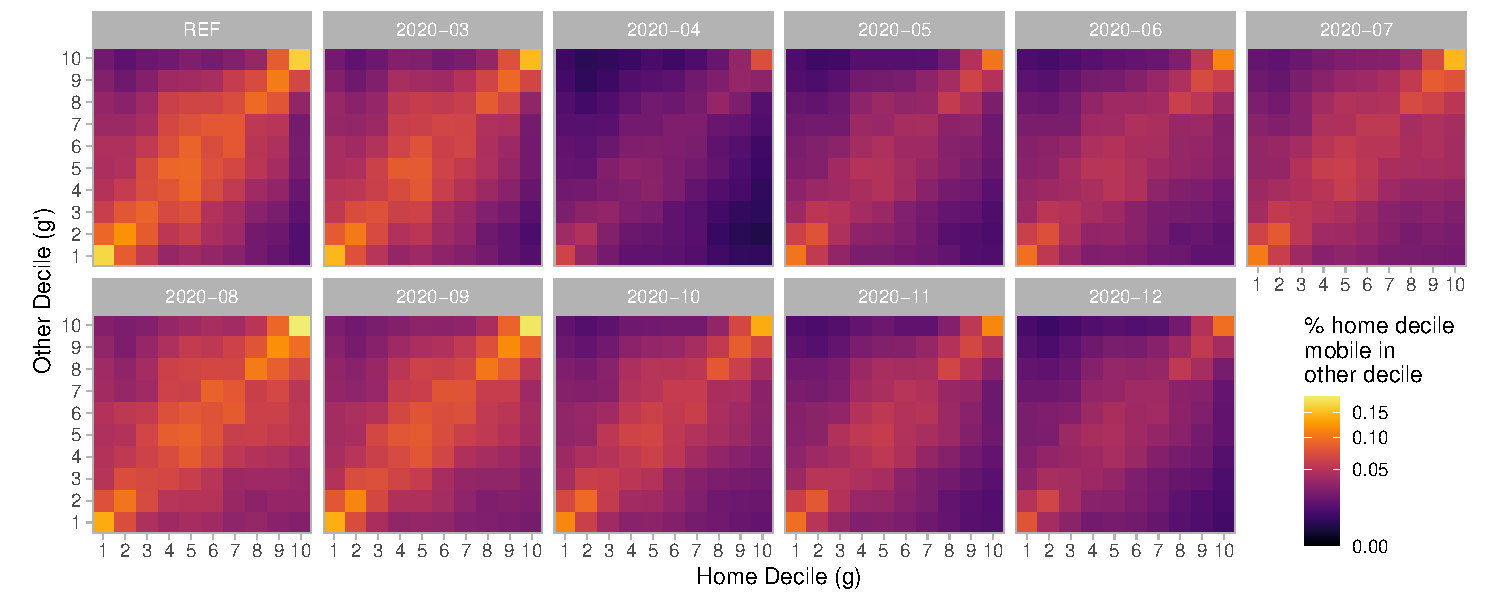
\includegraphics[width=\linewidth]{Bggit}
    \caption{Inter-FSA mobility}
    \label{fig:Bggot}
  \end{subfigure}
  \begin{subfigure}{\linewidth}
    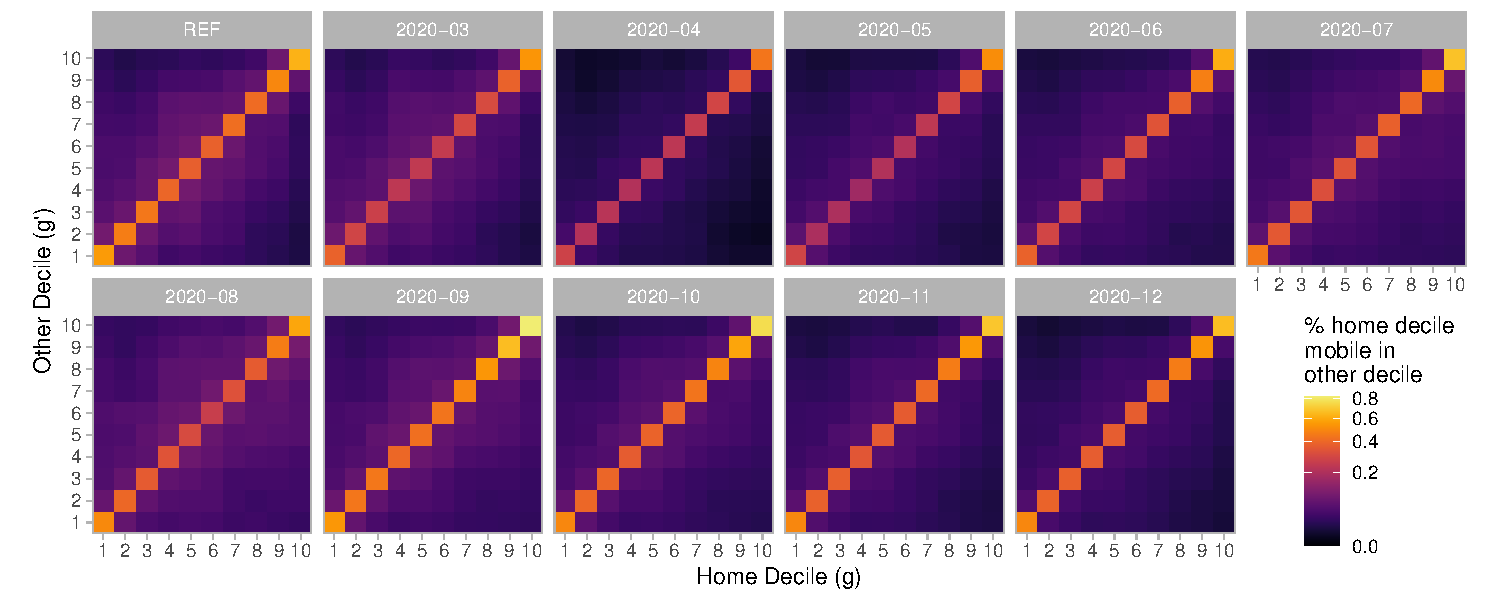
\includegraphics[width=\linewidth]{Bggt}
    \caption{Inter + intra-FSA mobility}
    \label{fig:Bggdt}
  \end{subfigure}
  \caption{Mobility matrix $B_{gg'}$, representing
    the expected proportion of individuals in decile (patch) $g$
    who are mobile in decile $g'$ per day,
    stratified by calendar month and the reference period}
  \label{fig:Bggt}
  \floatfoot{Derived from mobile device geolocation data;
    deciles represent groupings of Ontario forward sortation areas (FSAs)
    by cumulative \covid cases between Dec 2020--May 2021; % TODO: double check this period.
    colour scale is square-root transformed to improve perception of smaller values;
    reference period: Jan--Feb 2020.}
\end{figure}
\clearpage
% ==================================================================================================
\subsection{Additional Data for Ontario Patches}\label{app.covid}
\begin{figure}[ht]
  \centering
  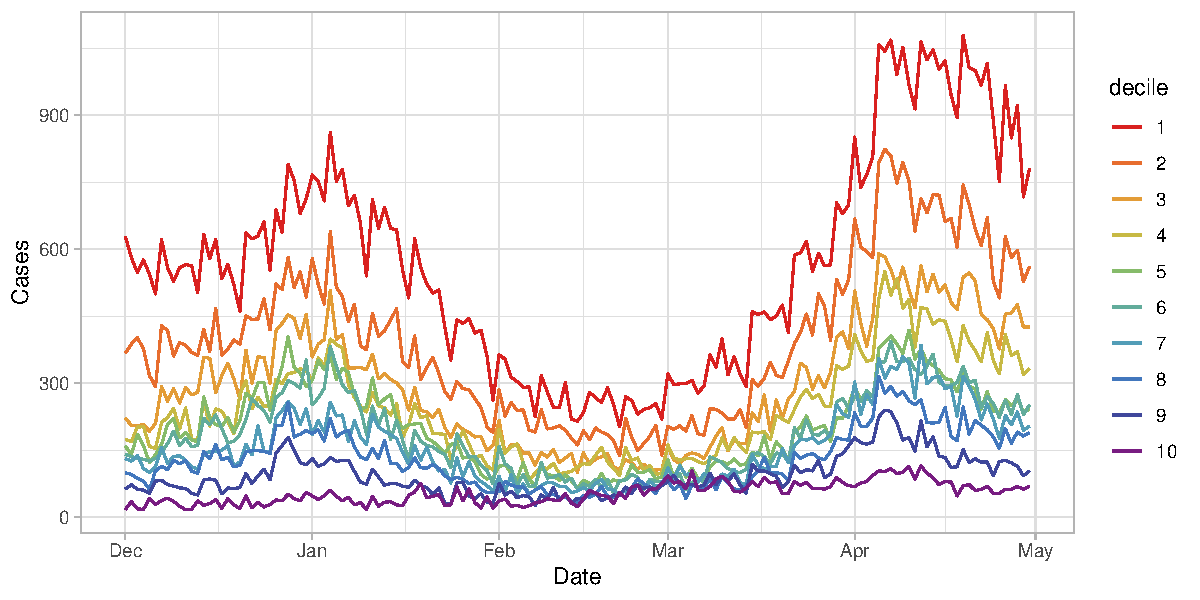
\includegraphics[width=.8\linewidth]{Yg}
  \caption{Time trends in daily \covid cases across the 10 deciles (patches) in Ontario}
  \label{fig:Yg}
  \floatfoot{Deciles represent groupings of Ontario forward sortation areas (FSAs)
    by cumulative \covid cases between Dec 2020--May 2021.} % TODO: double check this period.
\end{figure}
\begin{figure}[ht]
  \centering
  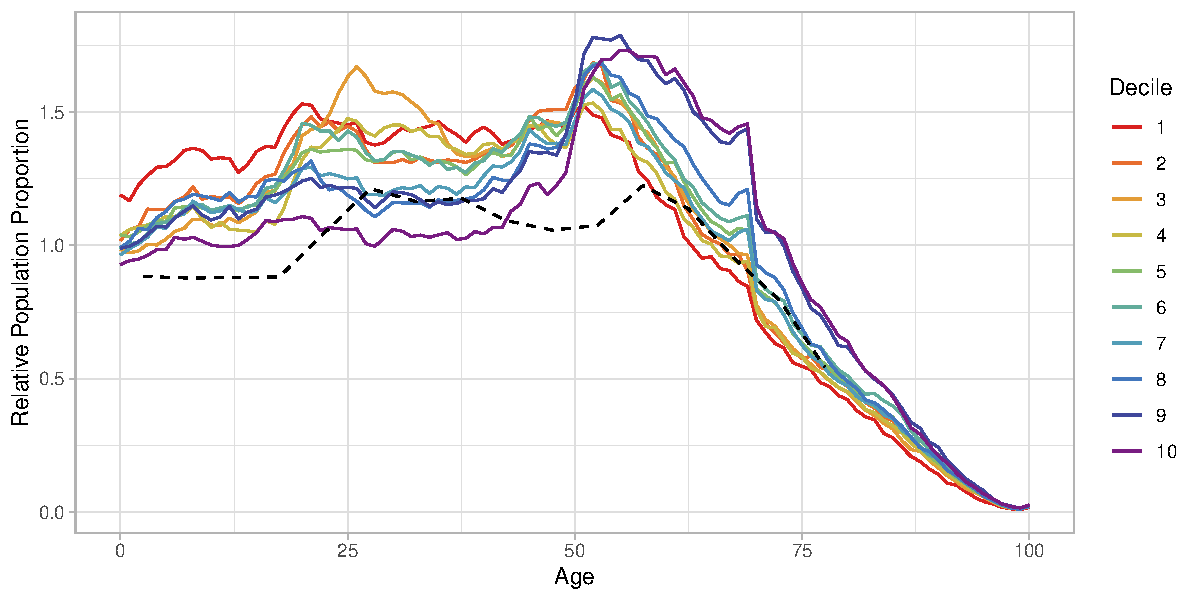
\includegraphics[width=.8\linewidth]{Pga}
  \caption{Population age distributions across the 10 deciles (patches) in Ontario}
  \label{fig:Pga}
  \floatfoot{Deciles represent groupings of Ontario forward sortation areas (FSAs)
    by cumulative \covid cases between Dec 2020--May 2021; % TODO: double check this period.
    solid coloured lines correspond to deciles;
    dashed black line corresponds to the Canadian age distribution used by \citet{Prem2017}.}
\end{figure}